\begin{figure}[tp]
\caption[Task outline]{
\emph{Task outline}
(A) A schematic of idealized categorical perception. \emph{Top green}: The psychometric function or the probability of classifying a stimuli as A or B as you move along a physical continuum between A and B. The category boundary occurs at the vertical red dotted line and there is some amount of uncertainty near this boundary. The boundary is defined as the point of perceived equality or the stimuli location on the physical continuum where a participant is equally likely to classify the stimuli as A or B. \emph{Top Blue}: is the discrimination curve describing how well a participant can discriminate between nearby stimuli. \CP has been described as a peak in the discrimination curve near the category boundary. The lower axis indicates how the perceptual space is stretched compared to the physical continuum causing stimuli that are within category limits to be perceived as closer than stimuli that lie across category boundaries, but are an equal distance apart.
(B) A diagram of the operant behavioral apparatus which consists of response ports with IR beak detection sensors, a food hopper to provide access to a food reward, and a speaker hidden behind the panel to present auditory stimuli.
(C) A diagram of generating an interpolating morph using a \DBN autoencoder. A spectrogram representation of two 400 ms song motif, A and D, are fed into a compressive network to create a latent representation, $Z_A$and $Z_D$. We then linearly interpolate between $Z_A$and $Z_D$ to create $Z_{ADmorph}$ which we can use to reconstruct a spectrogram motif that lies between A and D. Three example morph interpolations are shown below in (E)
(D) Diagram of the behavioral task. Spectrograms of the initial 8 randomly chosen 400 ms long motifs, labeled A-H, and their reward associated responses. Once the performance on these 8 reached a sufficient stable level, interpolated morph motifs, indicated by the 16 connecting lines were probed using a ratcheting double staircase procedure to allow the birds to determine their own behavioral boundaries.The 3 example morph dimensions displayed to the left are highlighted in blue.
(E) Three example interpolated morph dimensions generated using the \DBN. 16 (of 128 used) example motifs for each morph dimension. Spectrogram representation with frequency on y-axis and time on the x-axis. Each motif is 400 ms long.
\index{outline}}
\end{figure}

\begin{figure}[tbp] 
\contcaption{\emph{Task outline} Continued from previous page.}
  \centering
  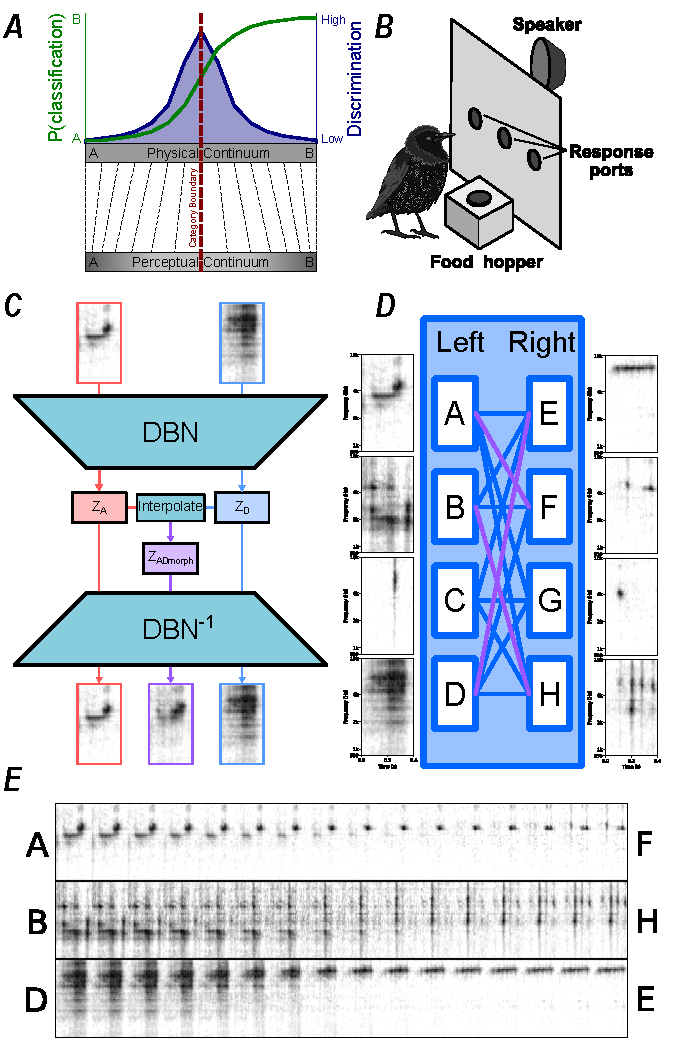
\includegraphics[width=114mm]{figures/fig01_task_outline.pdf}
  \label{fig:outline}
\end{figure}

\subsection{Generating smoothly varying morphs}

Using a large corpus of recorded starling song, a generative machine learning model is trained to non-linearly autoencode 400 mS motifs (song segments) of starling song in a low (64) dimensional latent space. The generative model attempts to model the distribution of song segments the model is trained on and as a result it tries to completely fill the latent space with projected representations due to an information bottleneck. The consequence of this is that for any point in the latent space, the spectrogram reconstruction of that point could lie within the actual distribution of starling song. Thus, the model can be used to interpolate between any two arbitrarily chosen starling motifs projected into the latent space to produce a smoothly varying continuum of morphed motifs that shift from one target motif to the other as outlined in \ref{fig:outline}(C). Instead of sounding like a simple linear crossfade between the two motifs, the network tries to produce a motif that could be in the distribution of recorded motifs, resulting in more realistic sounding motifs. Three examples of these smooth morphs are shown in \ref{fig:outline}(E) 

\subsection{Behavioral Measurement of Perceptual Space}

Using an operant behavioral apparatus diagrammed in \ref{fig:outline}(B), starlings are trained on a two alternative choice task where four arbitrarily chosen motifs (labeled A, B, C, and D) are associated with a left response and another four (E, F, G, and H), are associated with a right response as summarized in figure \ref{fig:outline}(D). After training to a stable performance criterion, the interpolated morph motifs generated by the \ac{DBN} are used to probe the bird's perception as each left-associated motif is transformed into each right-associated motif. We employed a ratcheting double staircase that \emph{allowed us to iteratively (and independently) estimate the categorical boundary along each of the 16 morph dimensions for each bird}. 

\subsection{Psychometric curves are conserved across subjects}

\begin{figure}[tp]
  \caption[Psychometric curves are conserved among different birds]{
  \emph{Psychometric curves are conserved among different birds}
(A)	Construction of a single psychometric curve: The x-axis represents presentations of stimuli that vary between motif A on the left and motif E on the right. The middle tick mark is the location of a stimuli that lies exactly between motif A and motif E (according to the \DBN). Thus the 3 tick marks indicate the location of stimuli that is (left) 75\% A, 25\% E, (middle) 50\% A, 50\% E, and (right) 25\% A, 75\% E. The y-axis is the probability of a right response (that has been operantly conditioned to be associated with motif E). The black dots represent the binary decision of the birds (responses are jittered to demonstrate relative density). All the responses ordered by morph position are binned into 16 equally sized bins and the 95\% confidence intervals of the mean estimates are plotted as vertical blue lines. The maximum-likelihood 4 parameter logistic fit of the probability of the bird responding right as a function of morph position between motif A and motif E, which we will call the psychometric curve, is plotted in blue.
(B)	Psychometric curve variation: The set of all 16 behaviorally determined psychometric curves for a single bird. Color indicates each of the 16 different morph dimensions.
(C-D)	Exemplar psychometric curves that are conserved between subjects: 2 of the 16 morph dimensions, (C) motif B to motif F and (D) motif A to motif H, are plotted for 4 different birds trained on the same categorization task. The full 16 dimensions are plotted in supplemental figure \ref{fig:psychometric-all}.
(E)	To measure how the B parameter (determines boundary sensitivity or slope at the boundary) of the psychometric curves is grouped we take the one-sided \KS metric between the distribution of pairwise distances between the B parameter of all psychometric curves, to the distribution of pairwise distances between the B parameter of psychometric curves from the same morph dimension (blue), and to the distribution of pairwise distances between the B parameter of psychometric curves from the same bird (red). The vertical blue line represents the \KS statistic between the distribution of pairwise distances between psychometric sensitivities that share the same morph dimension to that of all measured psychometric curves. The blue shaded cumulative survival curve is the distribution of expected \KS statistic values if we randomly split the psychometric curves into groups that share the same size as the morph dimension groups, or the null distribution as estimated by $2^{17}=131,072$ shuffles. Thus, the interception of the vertical blue line with the blue shaded cumulative survival curve provides an estimate of the likelihood that the psychometric sensitivities are as close to the psychometric sensitivities of other birds on the same morph dimension by chance, $p=3E-4$. We use an 8-way bonferroni correction to account for the 2 groupings and 4 parameters we test. * indicates $p<0.00625$, **, $p<0.00125$, and ***, $p<0.000125$. The vertical red line is the \KS statistic between the distribution of pairwise distances between psychometric sensitivities from the same bird to the distribution of pairwise distances between all psychometric sensitivities. Its corresponding shuffled null distribution is plotted as the red shaded region providing an estimate of $p=0.044$. Together, this indicates that psychometric sensitivities are closer than would be expected by chance when grouped by morph dimension, but not when grouped by bird. (continued on following page)
\index{conserved}}
\end{figure}


\begin{figure}[tbp] 
  \contcaption{
  \emph{Psychometric curves are conserved among different birds} Continued from previous page.
  (F)	The corresponding figure for the M parameter (boundary location). This shows that the likelihood that the psychometric boundaries are as close to the psychometric boundaries of other birds on the same morph dimension by chance (blue), $p<8E-6$ because never once in all the $2^{17}$ shuffles, was the KS statistic as great as the value measured. When distances between psychometric boundaries within a single bird are considered (red), $p=0.041$. This indicates that psychometric boundaries are also closer than would be expected by chance when grouped by morph dimension, but not when grouped by bird. Parameters A and K, the maximum accuracy achieved near each endpoint, are plotted in supplemental figure \ref{fig:AKconserved} and show the opposite trend.
}
  \centering
  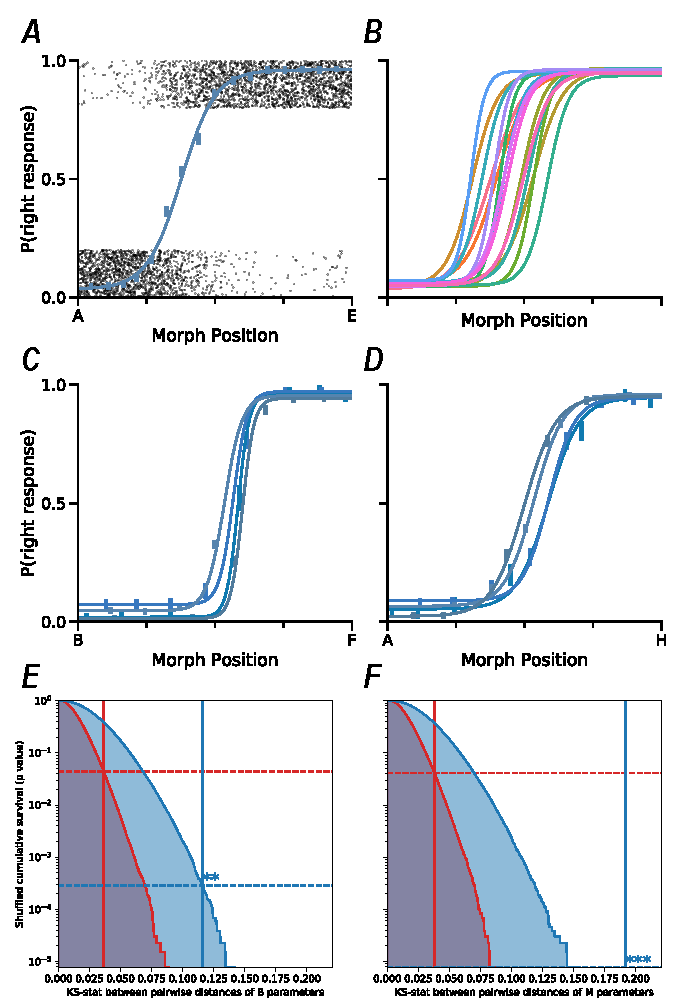
\includegraphics[width=114mm]{figures/fig02_conserved.pdf}
  \label{fig:conserved}
\end{figure}

This provides independent binary behavioral responses along each of the 16 possible dimensions interpolating from each of the 4 left associated motifs to each of the right associated motifs.

We fit a \textit{\textbf{psychometric curve}} of the form $P(R) = A + \frac{K - A}{1 + e^{-B(x-M)}}$ using maximum log likelihood for each of the 16 morph dimensions. $A$ and $K$ determine the maximum accuracy achieved near each endpoint. $M$ determines the boundary location or the point of subjective equality between each of the endpoints. $B$ determines boundary sensitivity or slope at the boundary.

A psychometric curve is fit to these behavioral responses and figure \ref{fig:conserved}(A) demonstrates how well a four parameter psychometric curve fits the average response along a single example dimension. We measure 16 of these curves for each bird.

In all cases, birds show very clear categorical perception as evidenced by the steepness each psychometric function regardless of bird or motif dimension. Comparing the psychometric curves within a single bird across all 16 motif-to-motif dimensions reveals a large amount of variation in the point of subjective equality (the category boundary) and in how sensitive the bird is to stimulus changes across the boundary (Fig. \ref{fig:conserved}(B)). This variability across dimensions is presumably a result of the non-linear nature of the \ac{DBN} song compression and morphing. Thus, we can conclude that \emph{the features the DBN uses to represent the motifs are perceptually relevant to the starlings}, and that the starlings are differentially sensitive to variation along these different feature dimensions.

Despite the significant variability within a single bird across multiple morph dimensions, we observed a remarkable degree of consensus between birds.  This included strong agreement in where each bird placed the category boundary on a given dimension, and in the sensitivity of all birds to changes along a given stimulus dimension (slope of psychometric function). Figure \ref{fig:conserved}(C-D) gives an example of the typical agreement between birds, where two of the 16 morph dimensions are plotted for 4 different birds.

Psychometric curves for four starlings, over several months of training, are highly conserved between individuals, suggesting a shared perceptual space. The y-axis shows the probability of a right response to a stimulus morphed continuously between, for example on the left, motif B (reinforced as left) and motif F (reinforced as right). The x-axis is the morph position between the left associated motif to the right associated motif.

$A$ and $K$, the left and right scaling parameters are statistically closer than would be expected when compared across all morphs within a single bird indicating that they are bird specific parameters as demonstrated by supplementary figure \ref{fig:???} and table \ref{tbl:???}. This makes sense because they correspond to the bird's absolute performance on the left and right endpoints. Figure \ref{fig:conserved}(E-F) and table \ref{tbl:???} also show that $M$, the category boundary and $B$, the sensitivity are conserved within the same morph dimension across different birds, but not within a single bird. This indicates the existence of a shared perceptual space of these synthetic natural-like sounds in these wild caught birds. 

\subsection{Different training context sometimes results in reliable shifts in the psychometric curves}

\begin{figure}[tbp] 
  \centering
  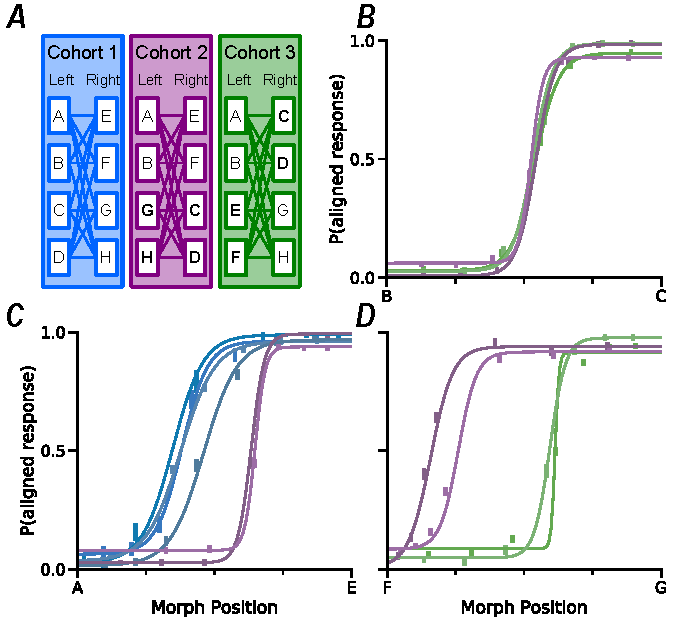
\includegraphics[width=114mm]{figures/fig03_shift.pdf}
  \caption[Different training context sometimes results in reliable shifts in the psychometric curves]
{
(A)	Diagram of alternative training contexts. Task structure remains the same in each cohort, but some motif category assignments change. Category assignment differences from Cohort 1 are bolded in Cohort 2 and 3. This allows a subset of the morph dimensions to be compared across training on different category permutations. Colors correspond to colors used in adjacent plots.
(B-D)	Exemplar psychometric curves from subjects trained on different category permutations. 
(B)	On most dimensions the boundary is conserved as if the training was the same as shown in the psychometric curves from these 4 birds, 2 from each of cohort 2 and 3 along the morph dimension between motif B and motif C. 
(C-D)	However, on some of the dimensions, such as A to E (left) and F to G (right), the behaviorally measured boundaries depend on the initial categorical assignment.  When there is a difference, the boundaries are still conserved within cohorts.
\index{shift}}
  \label{fig:shift}
\end{figure}

The shared perceptual space for motif categorization may result from either common training and experience, idiosyncrasies of the compressive network transformation, or some combination of the two. To test for this, we permuted the initial motif category assignments for a subset of birds. Instead of associating motifs A, B, C and D with left responses and motifs E, F, G, and H with right responses, a new cohort of birds learned, for example, to associate motifs A, B, E, and F with left responses and motifs C, D, G, and H with right responses. The category assignments for the three different cohorts are shown in figure \ref{fig:shift}(A). Thus, a subset of the 16 interpolating morph dimensions between left and right associated motifs is shared with the original cohort's interpolating morph dimensions. Comparing these shared boundaries demonstrates that on some of the interpolated morph dimensions, both cohorts of birds place the boundaries in same location as shown in figure \ref{fig:shift}(B) while in other interpolating morph dimensions each cohort has a separate boundary (but consistent within that cohort), as shown in figures \ref{fig:shift}(C-D). The boundaries that are preserved across motif category permutation indicate that these dimensions are independent from the other dimensions, however, the boundaries that are shifted as a result of the motif category permutation indicate an interaction between the interpolated morph dimensions. This is unexpected, especially if one considers that in the latent space of the DBN there is minimal collinearity and no discernable structure between any of the 8 motifs used.


\subsection{Electrophysiological Recordings}

To explore the neural underpinnings of categorical perception we record from secondary auditory regions of anesthetized starlings and present the generated motifs. We record from a total of 2019 neurons in <<<TODO>>> sites in 8 different starlings, 4 trained, 4 naive, never having heard the stimuli before. We use a 32 channel silicon electrode and stereotaxically target \ac{CMM} and \ac{CLM} as described in the methods and shown in figure \ref{fig}. We sort the data using MountainSort\cite{mountainsort}. 

\subsection{Single neurons have reliable temporally precise responses}

\begin{figure}[tp]
 \caption[Single neurons have reliable temporally precise responses]{
 \emph{Single neurons have reliable temporally precise responses}
(A)	Spectrogram representations of example stimuli presented to the anesthetized starlings of four example motifs presented, motifs A, B, F, and H.
(B) The equivalent audio waveform pressure representations. Black lines mark the start and end of the auditory stimuli.
(C) The raster plots of a single neuron for 240 presentations of each of these stimuli. Vertical marks are plotted at each time point of the occurrence of a spike in the 400 ms stimuli. The y-axis denotes the stimuli presentation. Black lines mark the start and end of the auditory stimuli.
(D) Average Gaussian convolved spike train representation in black. We convolve each individual trial with a Gaussian with $\sigma=10ms$ to get an instantaneous estimate of spike firing rate. These are plotted faintly to demonstrate trial to trial reliability and variance of this representation. The average of these 240 faint lines is plotted in black for each of these stimuli.
(E) Heatmap representation of the above representation to be used below. Lighter represents higher estimated instantaneous firing rate. These plots are all normalized to the max firing rate. The colored outlines indicate where the data is repeated below.
(F) Variation of the average Gaussian convolved single neuron’s representation across morph dimensions. Smoothly interpolated using triangulation for surface estimation. Morph position is plotted on the Y axis as the motif presented goes from motif A (highlighted in blue as a band along the bottom) to C (along the top) for example in the top left subplot. Time (during the stimuli presentation) is plotted on the X-axis. The representations of motif F (red) and motif H (Magenta) are diagrammed to demonstrate how the representation is using the average response of this neuron as the top row in the right two subplots in the top row of this representation. Other colors outline other areas that include the averaged representations from figure E.  Not all morph positions were presented the same number of times so confidence (not represented) varies along morph position axis.
\index{single}}
\end{figure}

\begin{figure}[tbp] 
\contcaption{\emph{Single neurons have reliable temporally precise responses} Continued from previous page.}
  \centering
  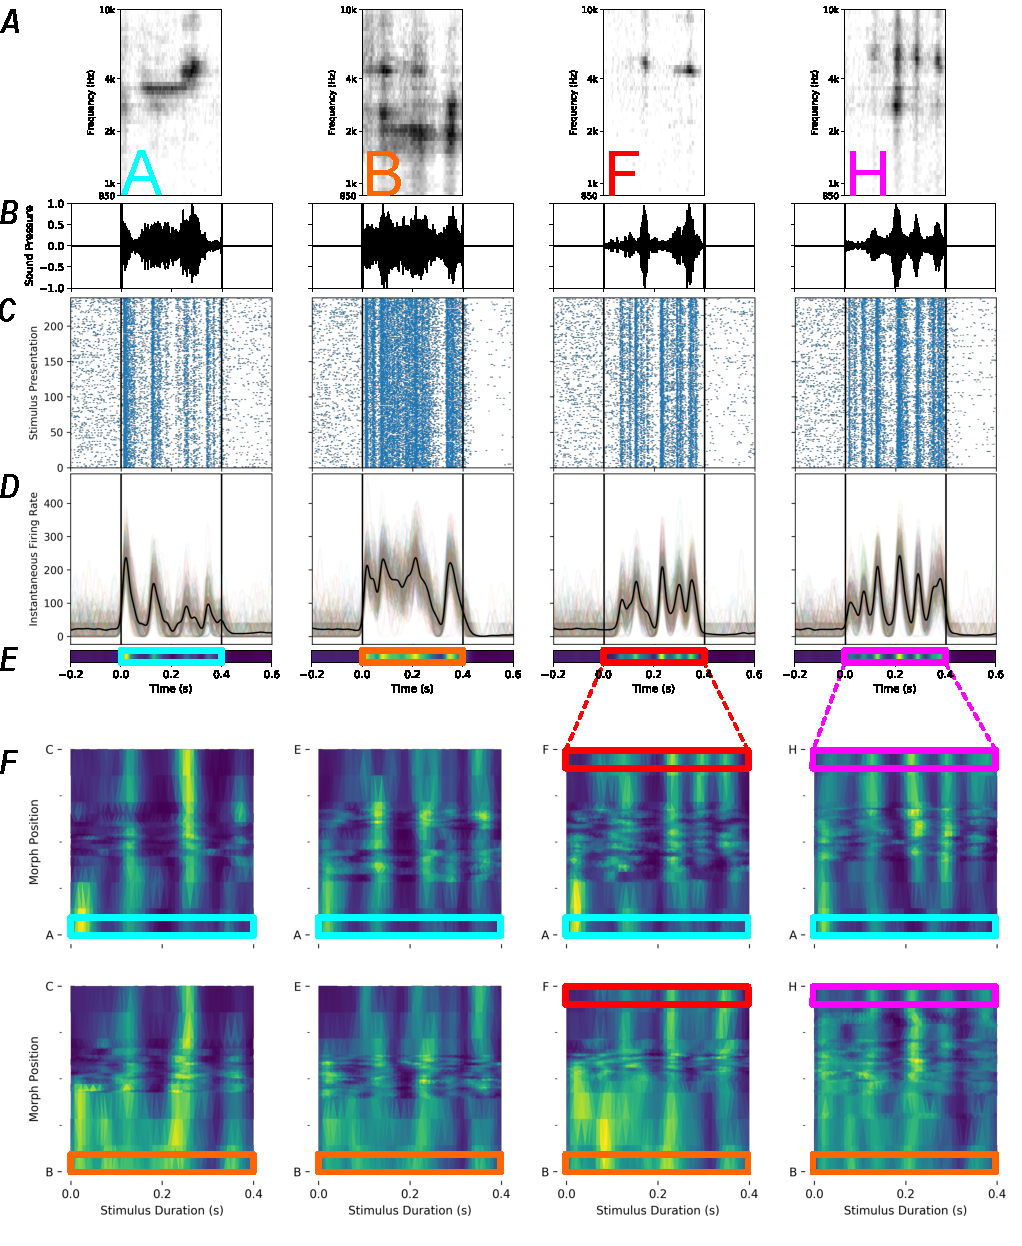
\includegraphics[width=\textwidth]{figures/fig05_single.pdf}
  \label{fig:single}
\end{figure}



We find the units are extremely time-locked and stimuli specific as demonstrated by figure \ref{fig}. Because of this we choose to include time in our neural representation by convolving the spike train with a Gaussian($\sigma = \SI{10}{ms}$). This provides us with a continuous estimate of firing rate through time for each trial for every unit. If we look at the average of this representation as we move along a morph dimension we find that there is a large amount of variation in how the units respond. Some units respond very smoothly to changes along a morph dimension, whereas others are quite categorical.

We restrict our analysis to units that are able to correctly identify the identity of our eight template motifs (averaged in a pairwise fashion so that 50\% is chance) more than 60\% of the time. This leaves 705 remaining "good" units as seen in figure \ref{fig}.

Using the hold-one-dimension-out prediction strategy, similar to that for the DBN activations, we predicted the behavioral psychometric functions from the neural population representations. The behavioral response is fit given the neural representation of stimuli presented from 15 of the 16 interpolated morph dimensions and then the response is predicted on the neural responses of the remaining dimension. For computational tractability we reduced the dimensionality of the neural representation to 24 dimensions using an LDA-like method. The mean squared error for each held out dimension are combined to provide 16 performances for each neural recording (39?) for each set of behaviorally determined psychometric fits (8). Once again we create a null distribution by shuffling the labels of the morph dimensions 2048 times and measuring the KS distance to distribution of 16 dimension performances. Overall we find the fits are significantly better than would we expected by chance. Furthermore, if we compare the distribution of p values for recordings from untrained naive birds against the recordings of the birds that had been behaviorally trained we find that there's no difference between how well the neural representation of naive birds or trained birds can predict the location of the boundary or the sensitivity to changes near the boundary. That is not to say that there is no difference between the population representation in trained or untrained birds, or that more information about boundary location isn't encoded elsewhere in the brain, but that the information that allows generalization of categorical boundary parameters to other morph dimensions is equally present in both trained and untrained birds.

\subsection{The $\partial N / \partial s$ Curve}

\begin{figure}[tbp] 
  \centering
  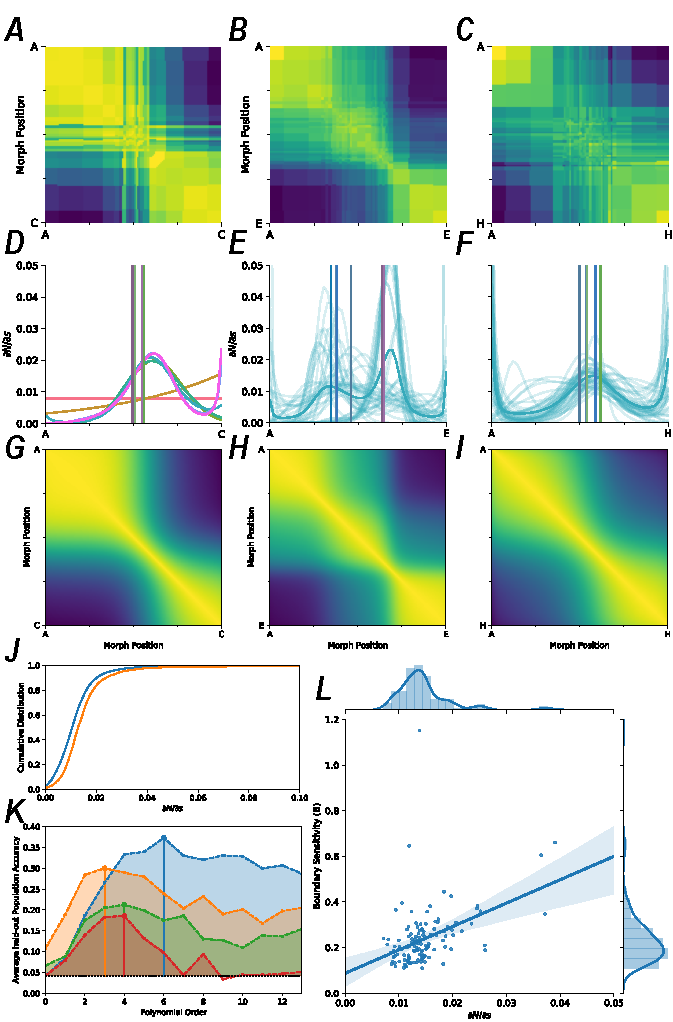
\includegraphics[width=114mm]{figures/fig07_derivative.pdf}
  \caption[The Thielk curve captures how neural representation changes as we move along a morph dimension]
{(continued on following page.)
\index{derivative}}
  \label{fig:derivative}
\end{figure}

\begin{figure}[tp]
  \contcaption{
(A)	The cross correlation matrix for a single recording on the morph dimension from motif A to motif C. Average cosine distance in the task relevant neural representation subspace between pairs of morph positions are initially calculated. These values are then upsampled to the full 128 pixel grid using nearest neighbor interpolation.
(B-C)	Average cross correlation matrix for all recordings (using the final stimuli set) for morph dimensions A to E and A to H.
(D)	Using a polynomial of order 0 through 6 to estimate the Thielk curve for a single recording and morph dimension, A to C (same as above).
Vertical lines represent the behaviorally determined psychometric boundaries for all birds tested across this morph dimension. The horizontal pink line is the 0th order fit, the exponential gold line is the 1st order fit.
(E-F)	4th order mean Thielk curves across all recordings on morph dimension AE (E) and AH (F). Individual 4th order Thielk curves for each recorded population are faintly plotted to show variance. Vertical lines represent the behaviorally determined psychometric boundaries for all birds tested across this morph dimension.
(G)	Cross correlation matrix reconstructed from the 4th order Thielk curve for the same recording used in (A) and (D).
(H-I)	Average reconstructed cross correlation matrix from all 4th order Thielk curves on AE (H) and AH (I)
(J)	Cumulative distributions of the value of the 4th order Thielk curve at psychometric boundary locations of the same dimension vs different dimensions as a control. A one-sided KS test provides a P value of $p=1.47E-121$
(K)	Average accuracy of predicting the morph dimension of a Thielk curve from a held out recorded neural population as we increase the order of the polynomial. The green and orange curves use the optimized polynomial coefficients to predict the morph dimension label. The red and blue curves use the normalized Thielk curve evaluated at 50 evenly spaced points along the morph dimension. The red and green curves use a multinomial logistic regression as the classification model. The orange and blue curves use XGBoost as the classification model. The vertical lines highlight the maximum average held-out prediction accuracy achieved by each method. Chance performance ($1/24$) plotted as a horizontal dotted line.
(L)	Correlation between the boundary sensitivity parameter (B) of the psychometric curve and the value of the 4th order Thielk curve for the given boundary location. Plotted above and to the right are the projected histograms and associated kernel density estimate of the distribution. Plotted as a line is the regression between these two variables with 1000 fold bootstrapped 95\% confidence interval plotted as a shaded region around the regression.
}
\end{figure}

We are interested in the brain's ability to discriminate changes along our morph dimension. We use distance in our neural representation to approximate the brain's ability to discriminate. 

We pose the following regression problem by defining the $\partial N / \partial s$ curve:
Given a stimuli representation space $S$ containing $\{s_i\}$ that lie along a 1D path $s$ and a neural representation space $N$ for a given recorded neural population where we have samples of noisy projection, through a brain, of examples of $s_i$ into $N$, which we will call $\mathcal{B}(s_i):s_i \to N$.
We would like to define the following curve as $T(s_i)=\frac{\partial N}{\partial s} (s_i): s_i \in s$, such that for a pair of presented stimuli, $s_i$ and $s_j$, and a distance, $y=|\mathcal{B}(s_i) - \mathcal{B}(s_j)|$ in neural representation space between these to presentations, $y = \int_{s_i}^{s_j}T(s)ds + \epsilon$ . This assumes that the neural representation of these stimuli smoothly vary (up to some noise) as I move along the morph dimension. We then perform the regression to minimize the \MSE of $\epsilon$ for all pairs of stimuli presented on a single morph dimension.

The $\partial N / \partial s$ curve measures how fast the neural representation changes as we move along a path in stimuli space. 

If we consider how the $\partial N / \partial s$ curve is related to the cross correlation matrices plotted in figure \ref{fig:derivative}(A-C), it is a function defined along the diagonal and the value of each $i,j$ is the distance $y$ fit by the integral of the function from $(i,i)$ to $(j, j)$. Figure \ref{fig:derivative}(G-I) show how much of the structure in the cross correlation matrices in (A-C) are described by the $\partial N / \partial s$ curves in (D-F)

We would like the $\partial N / \partial s$ curve $T(s_i)$ to have the following properties: 1. Strictly positive. 2. Smooth over the range $D$.
To keep the function positive I have used $T(s_i)=e^{f(x)}$ and to keep it smooth I have used $f(x)$ as a polynomial of varying orders.
Several other parameterizations have been explored but they provided qualitatively similar results and took significantly longer to fit.

The polynomial parameterization and $s_i$ sampling makes the $\partial N / \partial s$ curve highly susceptible to Runge's phenomenon near the ends of our morph dimension, especially for higher order polynomials. Therefore we do not interpret any spikes near the endpoints of our morph dimension as being meaningful.

Ignoring 0th and 1st order polynomial fits, higher order fits seem to all robustly fit the same curve shape as seen in figure \ref{fig:derivative}(D) with a peak near the behaviorally determined psychometric boundaries from other birds. This means that the neural representation was changing the fastest near the location on the morph dimension that other birds choose to place their boundary. This is less surprising when we see figure \ref{fig:derivative}(E-F) and see that the shape of the 4th order $\partial N / \partial s$ curve is fairly similar for every single neural population recorded. Thus the $\partial N / \partial s$ curve is a fairly recording invariant measure of changes in the neural representation. To statistically test this we try to predict the dimension a $\partial N / \partial s$ curve describes without seeing any other data from a recording in figure \ref{fig:derivative}(K). We use two different prediction models and two different representations of the $\partial N / \partial s$ curve and for each test our accuracy is much than the chance value of $1/24$. Each method-representation pair achieved max performance on held out populations using a polynomial order near a 4th order polynomial, which further reinforces are decision to use a 4th order polynomial fit. 

Lastly, if we consider the morph dimension from motif A to motif E (column BEH) where we observe a shift in the psychometric boundary between cohort 1 and 2, we see that many of the individual population $\partial N / \partial s$ curves have two peaks, and there is certainly two peaks in the average $\partial N / \partial s$ curve which correspond to the two locations of the psychometric boundaries.

If we compare the distribution of the value of the normalized $\partial N / \partial s$ curve at the psychometric boundary location for psychometric curves on the same morph dimension to the values for different morph dimension in figure \ref{fig:derivative}(J), we see a clear shift in the distribution and a 1-sided \KS test confirms this with a p-value of $p=1.47E-121$ indicating that it is very unlikely that morph dimensions boundaries do not occur at locations on the morph dimension with higher $\partial N / \partial s$ values than would be expected by chance.

Lastly, we use the natural variation in boundary location to test if greater $\partial N / \partial s$ values are correlated with greater boundary sensitivity (B) in the measured psychometric curves. The relationship in the average $\partial N / \partial s$ value of the psychometric boundary location to the boundary sensitivity (B) parameter has a Pearson's R correlation value of 0.42 which means we have a $p=6.5E-7$ that there is no correlation between these two variables.

\subsection{Predicting psychometric curves from neural population activity}
\begin{figure}[tbp] 
  \centering
  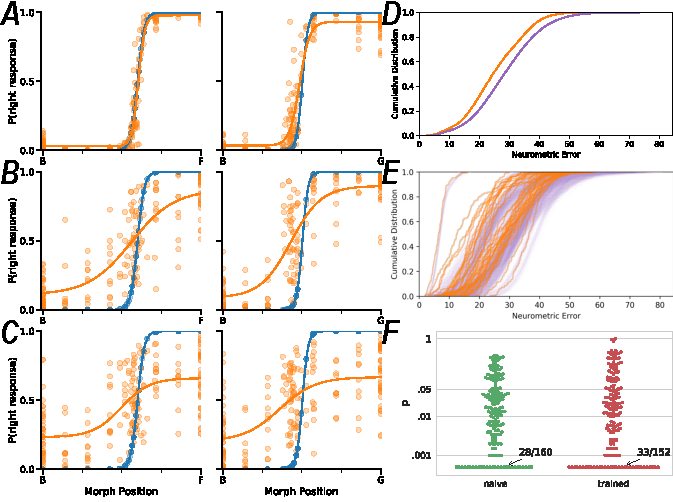
\includegraphics[width=114mm]{figures/fig08_neurometric.pdf}
  \caption[Predicting psychometric curves from neural population activity]
{
(A-C)   Predictions of behavioral psychometric curves for two morph dimensions, left: B to F, right:B to G, for the same behavioral bird, using three different recorded neural populations of differing quality. (A) shows an excellent fit, (B) shows a good fit, and (C) shows a fair fit for these two morph dimensions. Plotted in blue is the behavioral target, and plotted in orange are the held out predictions from a logistic regression trained on the other $15/16$ morph dimensions. The orange dots are the predicted probability of each stimuli presentation and the orange line is a 4 parameter logistic curve fit using \MSE to the probabilities. Some populations (A) do a lot better job at predicting the psychometric curves than others (C).
(D) Cumulative Distribution of the \MSE for neural predictions of the psychometric functions in orange and the cumulative distribution of the \MSE for neural predictions of shuffled psychometric functions in purple. This is the complete cumulative distribution for the \MSE for each of the 16 dimensions, for predictions against the psychometric curves of each behavioral bird (8), for all recorded neural populations (39).
(E) Same as (D) except plotted individually for each neural population in orange, and individually for each of 64 shuffles in purple.
(F) Shuffling each population against the behavioral curves 2048 times and comparing the \KS metric between the distributions allows us to estimate the p values for each neural population. Overall we find most population fits to perform better than would be expected by chance. Furthermore, if we split the recorded populations depending on whether they were from birds trained on this task or naive (never having heard the stimuli before) we find no difference in the distribution of p values. That is to say that a \KS test between the distribution of p values obtained for trained birds against the distribution of p values obtained for naive birds fails to reject the null hypothesis with a p value of $p=0.565$.
\index{neurometric}}
  \label{fig:neurometric}
\end{figure}